To evaluate the performance of our system we perform experiments that draw comparisons in terms of quantitative pose estimation and qualitative reconstruction quality and efficacy.
Firstly, pose estimation is evaluated against a well established dense SLAM system \cite{Prisacariu2014}, with the primary difference being that in the benchmark system, the entire 
visible scene is used for pose estimation, whereas in our system only the object is tracked.
Qualitative comparisons are also drawn between the reconstructions of our system versus those of the system described in \cite{Ren2013}.

We evaluate the system on a set of objects of different sizes, some sequences with the object moving, others with the camera moving. However, it should be noted that in the case of the 
comparisons with the dense SLAM system it is not possible to evaluate the object motion sequences due to the tracking of the entire scene. Object motion with a static scene in this case 
would serve only to corrupt the scene model and tracking results, due to the systems inability to handle dynamic scenes.

\subsection{Pose Estimation Quality}
In this section we present quantitative results of our systems ability to maintain tracking robustness when tracking only an object and not the scene. In addition, the outputted trajectories 
of our system demonstrate less tracking drift and a robustness to loop closure events. We evaluate on <N> sequences of objects where the motion is restricted to camera only for the reason 
previously outlined. At this point it should be highlighted that the benchmark system has the advantage of an increased amount of geometry from which instantaneous poses can be estimated.
In the following experiments tracking is performed using only geometry cues from the rendered models and instantaneous depth frame.\\

Tracking between the two systems is evaluated w.r.t. ATE(Absolute Trajectory Error) as outlined in \cite{sturm12iros} and is summarised in Table \ref{ateTable}
\begin{table}[!t]
	{\small
		\begin{center}
			\begin{tabular}{l@{\hskip 1cm} c c}
				\emph{Sequence Name} & \emph{ATE}\\
				\midrule
				\textsf{Chair} & 0.048197\\
			\end{tabular}
		\end{center}
	}
	\caption{The absolute trajectory error (ATE) results (in metres, lower is better) achieved by our approach in comparison to the baseline InfiniTAM.}
	\label{ateTable}
\end{table}

\begin{figure*}[!t]
	\centering
	\caption{Trajectories outputted by the InfiniTAM dense SLAM system and our system.}
	\begin{subfigure}[b]{0.3\textwidth}
		\centering
		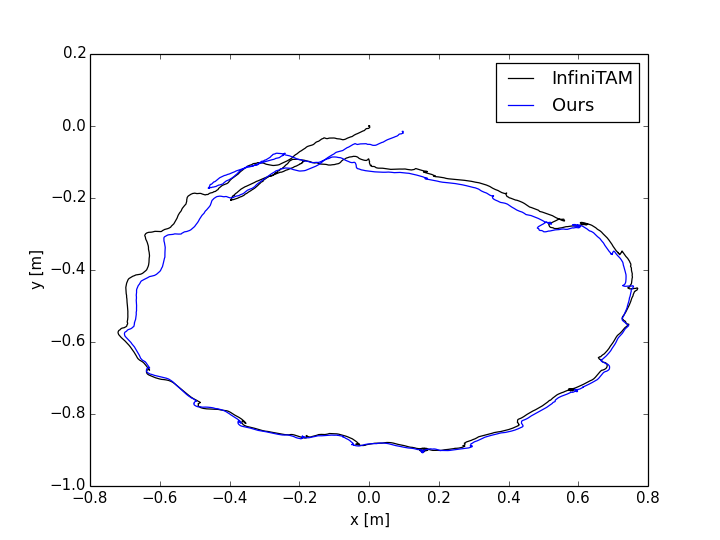
\includegraphics[scale=0.25]{plots/chairTrajectories.png}
		\caption{Chair Sequence}
		\label{chairTrajectory}
	\end{subfigure}%
	\begin{subfigure}[b]{0.3\textwidth}
		\centering
		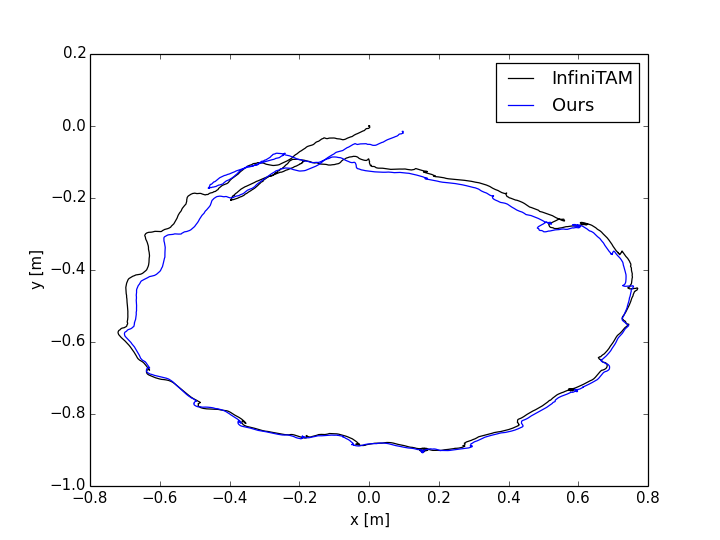
\includegraphics[scale=0.25]{plots/chairTrajectories.png}
		\caption{Chair Sequence}
		\label{chairTrajectory2}
	\end{subfigure}%
	\begin{subfigure}[b]{0.3\textwidth}
		\centering
		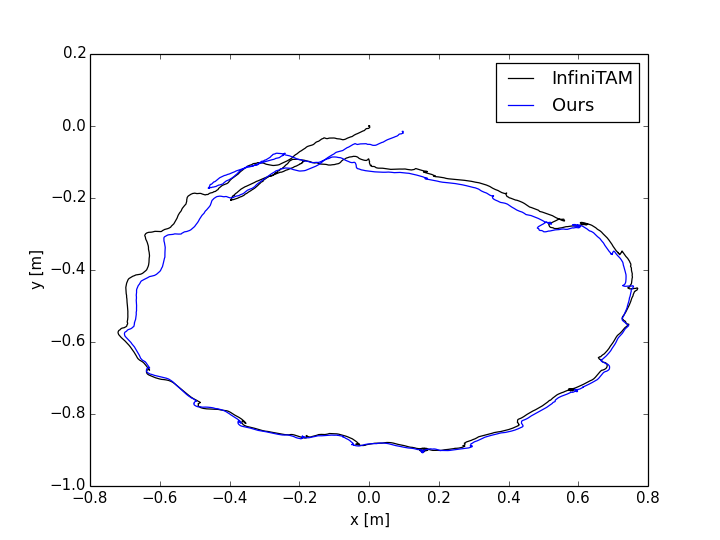
\includegraphics[scale=0.25]{plots/chairTrajectories.png}
		\caption{Chair Sequence}
		\label{chairTrajectory3}
	\end{subfigure}
\end{figure*}

\subsubsection{Chair Sequence}
In this sequence a static chair is reconstructed by moving the camera in an approximately circular fashion around with some repetitive camera motion at the end of the sequence to test 
the loop closure ability of the systems. The outputted trajectories may be found in Figure \ref{chairTrajectory}.
As can be seen in figure \ref{chairTrajectory} the robustness deficit when tracking with significantly is minimal, with the benchmark system appearing to incur cumulative tracking drift, as can be seen 
by the outwards `spiral' effect in the trajectory plots. In terms of overall ATE, the comparison between the two systems yields an ATE of \textbf{0.048197}.

\subsubsection{Cat Ornament Sequence}
%

\subsubsection{Teddy Sequence}